\subsection{Ray Casting}
\label{subsec:ray_casting}

\todo[inline]{Expand this section. Add formulas as well as examples.}
\todo[inline]{Punkte mehr ausführen; Integration zeigen mit Diskretition; auch Berechnungen}

Bei \textbf{Ray Casting} handelt es sich grundsätzlich um eine Strategie zur
Simulation, wieviel Licht anhand eines (Licht-) Strahles zu der sichtbaren
Bildfläche (also dem Betrachter) transportiert wird.

Das Verfahren wurde erstmals 1968 in~\cite{appel_techniques_1968}
vorgeschlagen und auch 1968 von der Matthematical Applications Group
Inc.\ in~\cite{arlington_mathematical_applications_group_inc_afips_1968}
erfolgreich umgesetzt.

Ein möglicher Algorithmus, wie Ray Casting umgesetzt werden kann, findet
sich in~\ref{fig:ray_casting:high_level}.

Es wird ein ``Projektionszentrum'' (das Auge eines Betrachters) sowie
eine Region einer beliebigen Bildfläche gewählt. Dabei kann die Region
als gerasterte Fläche angenommen werden. Jedes Raster entspricht den
Bildpunkten (Pixeln) der gewünschten Auflösung.  Daher, je feiner die
Rasterung, desto höher die Auflösung.

Für jeden Bildpunkt der gewählten Region wird ein Strahl
generiert, welcher dann vom Projektionszentrum durch das Zentrum des
Bildpunktes auf die Szene ``geworfen'' wird. 

Es wird dann das Objekt gesucht, welches den nähesten Schnittpunkt mit
dem Strahl bildet. Für jede Lichtquelle der Szene wird geprüft, ob die
Lichtquelle vom Schnittpunkt aus sichtbar ist. Ist dies der Fall, wird
schliesslich die Farbe und die Farbintensität an diesem Schnittpunkt
anhand eines Beleuchtungsmodelles (z.\ B.\ dem Phong-Beleuchtungsmodell)
berechnet. Ansonsten befindet sich der Punkt im Schatten, wird also
nicht beleuchtet.

\begin{figure}[H]\label{fig:ray_casting_illustration}
    \centering
    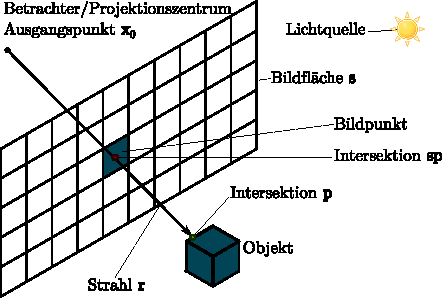
\includegraphics{img/ray_casting.pdf}
    \caption{Illustration des Ray Casting Verfahrens\protect\footnotemark}
\end{figure}
\footnotetext{Eigene Darstellung mittels Inkscape}

Die obenstehende Darstellung~\ref{fig:ray_casting_illustration} zeigt
das Prinzip des Ray Castings. Ausgangspunkt bildet der Betrachter mit
$x_{0} = (x_{x_{0}}, y_{x_{0}}, z_{x_{0}})$. Es wird ein Strahl $r = (x_{0}, d)$
in Richtung $d$ der Bildfläche $s$ ``geworfen''. Der Strahl $r$
schneidet die Bildfläche $s$ an einem Punkt $S = (x_{S}, y_{S}, z_{S})$.
Somit ergibt sich die Richtung $d = S - x_{0} = (x_{S} - x_{x_{0}},
y_{S} - y_{x_{0}}, z_{S} - z_{x_{0}}) = (x_{d}, y_{d}, z_{d})$. Der
Strahl $r$ trifft und schneidet schliesslich ein Objekt am Punkt $p =
r(t) = x_{0} + t \cdot d$ wobei $t \int [1, \infty]$ ist. Dies führt dazu, dass das
Raster, durch welches der Strahl $r$ hindurch geht, die Farbe des
getroffenen Objektes annimmt.

\subsubsection{Berechnung von Schnittpunkten}
\label{ssubsec:ray_casting_intersections}

Um den Schnittpunkt eines Lichtstrahles mit einem Objekt zu berechnen
wird grundsätzlich die mathematische Gleichung des Lichtstrahles in die
des Objektes eingesetzt. Existiert eine reelle Lösung, so schneidet der
Lichtstrahl das Objekt am nähesten Punkt zwischen dem Schnittpunkt und
der Oberflächennormale des Objektes.

~\citeauthor{glassner_introduction_1989} beschreibt mehrere Methoden zur
Prüfung von Schnittpunkten, hier sei beispielhalber nur die Intersektion
mit einer Kugel sowie mit einem Dreieck genannt.

Um den Schnittpunkt bzw.\ die Schnittpunkte eines Lichtstrahles mit
einer Kugel zu erhalten, wird die Gleichung des Lichtstrahles:

\begin{gather}
    r(t) = r_{0} + t \cdot r_{d}
\end{gather}

in die implizite Gleichung einer Kugel:

\begin{gather}
    \|\bm{x} - c\|^{2} - r^{2} = 0
\end{gather}

eingesetzt:

\begin{align}
    \|r(t) - c\|^{2} - r^{2} &= 0 \\
    \|r_{0} + t \cdot r_{d} - c\|^{2} - r^{2} &= 0
\end{align}

Das Auflösen dieses Gleichungssystemes ergibt folgende Fälle:
\begin{itemize}
    \item{Zwei Lösungen}: Der Strahl geht durch die Kugel hindurch.
    \item{Eine Lösungen}: Der Strahl streift die Kugel an einem Punkt
        als Tangente.
    \item{Imaginäre Lösung}: Der Strahl verfehlt die Kugel komplett.
\end{itemize}

Um den Schnittpunkt eines Lichtstrahles mit einem Dreieck zu erhalten,
wird die Gleichung des Lichtstrahles:

\begin{gather}
    r(t) = r_{0} + t \cdot r_{d}
\end{gather}

als Lösung der Gleichung eines Dreiecks mit baryzentrischen Koordinaten:

\begin{gather}
    x(\beta, \gamma) = v_{1} + \beta(v_{2} - v_{1}) + \gamma(v_{3} - v_{1})
\end{gather}

verwendet:

\begin{align}
    r_{0} + t \cdot r_{d} &= v_{1} + \beta(v_{2} - v_{1}) + \gamma(v_{3} - v_{1})
\end{align}

Der Lichtstrahl schneidet das Dreieck genau dann, wenn gilt $\beta +
\gamma \le 1$, $\beta \ge 0$ und $\gamma \ge 0$.

Es ist leicht verständlich, dass es sehr aufwändig ist jegliche Objekte
auf Schnittpunkte zu testen (so wie in
Beispiel~\ref{fig:ray_casting:high_level}). So wurde eine Vielzahl an
Methoden entwickelt um dies zu Beschleunigen. Eine Möglichkeit ist es
das Finden der Schnittpunkte zu Beschleunigen, z.B. durch Verwendung von
Hüllköpern, oder die Anzahl der Berechnungen zu minimieren, z.B. durch
Verwendung von Objekthierarchien oder der Unterteilung des Raumes einer
Szene. Das Kapitel ``A Survey of Ray Tracing Accelelration
Techiques''~\cite{glassner_introduction_1989}[S. 202ff] bietet einen
guten Überblick.

\begin{lstlisting}[language=Python,caption={Eine abstrakte Umsetzung des Ray
        Castings\protect\footnotemark.},label={fig:ray_casting:high_level},captionpos=b,emph={ray_cast}]
def ray_cast():
    # "pixels" is a list of all pixels of the image plane
    for pixel in pixels:
        # Save all intersections for given pixel
        intersections = []

        # Returns the ray passing through the given
        # pixel from the eye
        ray = ray_at_pixel(pixel)

        # "scene_triangles" is a list of all triangles
        # coming from meshes contained in the scene to render
        for triangle in scene_triangles:
            p   = intersect(ray, triangle)
            sum = 0

            for light in incoming_lights_at_p:
                sum = sum + l.value
            end

            if is_smallest_intersection(p, intersections):
                pixel = sum
            intersections.append(p)
\end{lstlisting}
\footnotetext{Algorithmus in Pseudocode gemäss~\cite{hughes_computer_2013}[Kapitel 15, Seite 391, Auflistung 15.2]}

